
Most of the data about the skew quadrupole was presented in Section~\ref{subsection: 1d_quench_propagation_geometry}. Unlike to 1D analyses presented in previous chapters, when a 3D thermal simulation of a magnet is considered, it is important to specify its reeling scheme because the windings interact with each other thermally across the insulation layer. Fig.~\ref{fig:skew_quad_transversal_cross_section} shows the transversal cross-section of one quadrants of the skew quadrupole. The windings are enclosed within an area of 24.5x27.3~mm. Moreover, each quadrant is covered with a 1 mm-thick ground insulation layer apart from the insulation between each winding described in Section~\ref{subsection: 1d_quench_propagation_geometry}. The internal side of the quadrant is thinner and accounts for 0.15~mm.

\begin{figure}[H]
    \centering
    \begin{tikzpicture}
    \pgftext{\includegraphics[width=\linewidth]{sections/skew_quad_q_det/figures/skew_quad_transversal_cross_section.png}} at (0,0);
    \node[red] at (6.0,2.1) {layers};
    \node[red, rotate=90] at (4.3,0) {turns};
    \draw[red, very thick, dashed] (0.47,-0.95) -- (0.47,2.4); 
    \node[red, scale=0.8] at (1.9,2.1) {quadrant symmetry};
    \draw[black, very thick, ->] (-4.3,2.1) -- (-4.8,1.8); 
    \node[black, scale=0.8] at (-3.0,2.1) {ground insulation};
    \end{tikzpicture}
    \caption{The transversal cross-section of one quadrant of a skew quadrupole~\cite{marco_prioli_mails}.}
    \label{fig:skew_quad_transversal_cross_section}
\end{figure}

As shown in Fig.~\ref{fig:winding_arrangement_cross_section}, each quadrant has 29 turns in each of its 26 layers. In total, the number of windings per quadrant is 754~\cite{hl_lhc_tech_design_report_v01, marco_prioli_mails}.

\begin{figure}[H]
\centering
    \begin{tikzpicture}
        \begin{axis}[
          width=0.5\linewidth, 
          height=0.5\linewidth,
          xtick={0.0, 24.46},
          ytick={0.0, 27.30},
          xlabel={$x,~\text{mm}~\text{(layers direction)}$},
          ylabel={$y,~\text{mm}~\text{(turns direction)}$},
          xmajorgrids=true,
          ymajorgrids=true,
          xmin=-5.0,
          xmax=29.47,
          ymin=-5.0,
          ymax=32.29,
          ]
          \addplot[blue, only marks, mark size=1pt] table[x=x,y=y,col sep=comma] {sections/skew_quad_q_det/figures/winding_location_cross_section.csv};
        \end{axis}
        \draw[scale=0.172, red, very thick, dashed] (2.5,2) -- (2.5,33.0); 
        \node[red, scale=0.8] at (1.9,5.6) {quadrant symmetry};
        
    \end{tikzpicture}
    \caption{Location of the windings in the cross-section of a half-quadrant.}
    \label{fig:winding_arrangement_cross_section}
\end{figure}

The winding scheme is shown in Fig.~\ref{fig:winding_scheme_cross_section}. The winding~1 occupies the region close to the position~(0,0). The last winding number 754 is placed further in x-direction. The \nth{2} half of each quadrant is a~mirror reflection of the presented winding scheme.

\begin{figure}[H]
\centering
    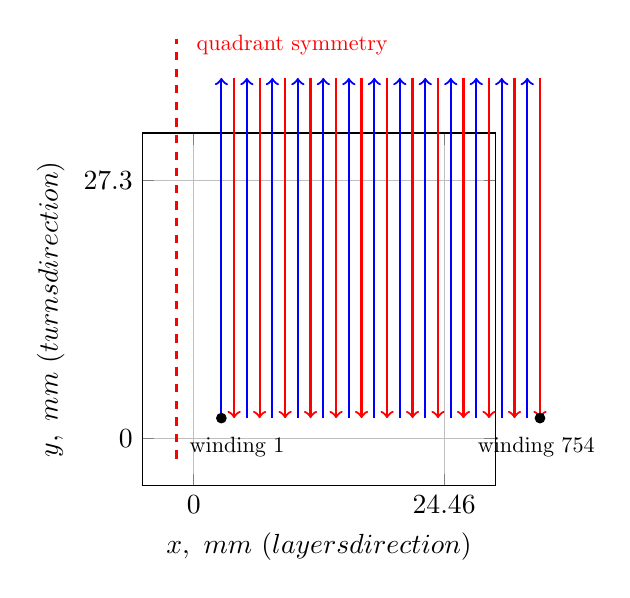
\begin{tikzpicture}
        \begin{axis}[
          width=0.5\linewidth, 
          height=0.5\linewidth,
          xtick={0.0, 24.46},
          ytick={0.0, 27.30},
          xlabel={$x,~\text{mm}~\text{(layers direction)}$},
          ylabel={$y,~\text{mm}~\text{(turns direction)}$},
          xmajorgrids=true,
          ymajorgrids=true,
          xmin=-5.0,
          xmax=29.47,
          ymin=-5.0,
          ymax=32.29,
          ]
        \end{axis}
        \foreach \t in {0.471, 2.353,...,24}
            \draw[scale=0.172, blue, thick, ->] (\t+5.35,5.0) -- (\t+5.35,26.819+3.3); 
        \foreach \t in {1.412, 3.294,...,25}
            \draw[scale=0.172, red, thick, ->] (\t+5.35,26.819+3.3) -- (\t+5.35,5.0);
        \draw[scale=0.172, red, very thick, dashed] (2.5,2) -- (2.5,33.0); 
        \node[red, scale=0.8] at (1.9,5.6) {quadrant symmetry};
        \filldraw[scale=0.172, black] (0.471+5.35,5.0) circle (10pt);
        \node[black, scale=0.8] at (1.2,0.5) {winding 1};
        \filldraw[scale=0.172, black] (23.996+5.35,5.0) circle (10pt);
        \node[black, scale=0.8] at (5.0,0.5) {winding 754};
        
    \end{tikzpicture}
    \caption{Winding scheme of a quadrant of a skew quadrupole.}
    \label{fig:winding_scheme_cross_section}
\end{figure}

The general parameters of the skew quadrupole are summarised in Table~\ref{table:skew_quad_params_table}. In the given magnet, there is only one aperture which a particle beam travels through. There is also one circuit used to power all quadrants of the magnet. It is interesting to mention that the coil length of only one quadrant is more than 800~m which is a very large number for thermal quench simulations, as mentioned in Section~\ref{subsection: 1D_quench_propagation_conclusions}. The operating current of the skew quadrupole is $I=182~\text{A}$.

\begin{table}[H]
    \caption{Geometrical parameters for skew quadrupole \cite{hl_lhc_tech_design_report_v01, marco_prioli_mails}} 
    \vspace{-1.em} 
    \fontsize{10}{10}
    \selectfont 
    \renewcommand{\arraystretch}{1.5}
    \begin{center}
    \begin{tabular}{ ccc }  
    \hline
    number of apertures & 1 & [-] \\
    number of circuits & 1 & [-] \\
    aperture size & 150 & [mm]\\
    coil length/quadrant & 841 & [m] \\
    operating current & 182 & [A] \\
    \hline 
    \end{tabular}
    \end{center}  
     \label{table:skew_quad_params_table} 
 \end{table}